\documentclass[12pt]{report}
\usepackage[utf8]{inputenc}
\usepackage[T2A]{fontenc}
\usepackage[russian]{babel}

\usepackage{amsmath,amsfonts,amssymb,amsthm,mathtools}
\DeclarePairedDelimiter\abs{\lvert}{\rvert}

\usepackage{pgfplots}
\usepackage{filecontents}
\usepackage{indentfirst}
\usepackage{eucal}
\usepackage{enumitem}
% Для \abs{}
\usepackage{commath}
\usepackage{float}
\frenchspacing

% Для нормальных переносов
\sloppy

\usetikzlibrary{datavisualization}
\usetikzlibrary{datavisualization.formats.functions}

\usepackage[left=2cm,right=2cm, top=2cm,bottom=2cm,bindingoffset=0cm]{geometry}
% Для измененных титулов глав:
\usepackage{titlesec, blindtext, color} % подключаем нужные пакеты
\definecolor{gray75}{gray}{0.75} % определяем цвет
\newcommand{\hsp}{\hspace{20pt}} % длина линии в 20pt
% titleformat определяет стиль
\titleformat{\chapter}[hang]{\Huge\bfseries}{\thechapter\hsp\textcolor{gray75}{|}\hsp}{0pt}{\Huge\bfseries}

% plot
\usepackage{xcolor}
\usepackage{stmaryrd}
\usepackage{wasysym}
\usetikzlibrary{datavisualization}
\usetikzlibrary{datavisualization.formats.functions}

% листинги
\usepackage{listings}
\usepackage{graphicx}
\usepackage{caption}
\usepackage{textcomp}
\lstset{
    language = Python,
    basicstyle=\small\sffamily,
    numbers=left,
    numberstyle=\tiny,
    stepnumber=1,
    numbersep=5pt,
    showspaces=false,
    showstringspaces=false,
    showtabs=false,
    frame=single,
    tabsize=2,
    captionpos=t,
    breaklines=true,
    breakatwhitespace=false,
    escapeinside={\#*}{*)}
}
\captionsetup[lstlisting]{justification=raggedright, singlelinecheck=off}

\addto\captionsrussian{% Replace "english" with the language you use
	\renewcommand{\contentsname}%
	{Содержание	}%
}

\begin{document}
%\def\chaptername{} % убирает "Глава"
    \include{title}
    \tableofcontents

    % Введение
    \newpage
    \chapter*{Введение}
    Конвейер — способ организации вычислений, используемый в современных процессорах и контроллерах с целью повышения их производительности (увеличения числа инструкций, выполняемых в единицу времени — эксплуатация параллелизма на уровне инструкций), технология, используемая при разработке компьютеров и других цифровых электронных устройств.
    
    Сам термин <<конвейер>> пришёл из промышленности, где используется подобный принцип работы — материал автоматически подтягивается по ленте конвейера к рабочему, который осуществляет с ним необходимые действия, следующий за ним рабочий выполняет свои функции над получившейся заготовкой, следующий делает ещё что-то. Таким образом, к концу конвейера цепочка рабочих полностью выполняет все поставленные задачи, сохраняя высокий темп производства. Например, если на самую медленную операцию затрачивается одна минута, то каждая деталь будет сходить с конвейера через одну минуту. В процессорах роль рабочих исполняют функциональные модули, входящие в состав процессора.
    
    \section*{Цель лабораторной работы}
    Целью данной работы является реализация асинхронного взаимодействия потоков на примере конвейерной обработки данных.
    
    \section*{Задачи лабораторной работы}
    
   В рамках выполнения работы необходимо выполнить следующие задачи:
    \begin{itemize}
    	\item Изучить асинхронное взаимодействие на примере конвейерной обработки данных.
    	\item Привести схему конвейерных вычислений.
    	\item Описать используемые структуры данных.
    	\item Определить средства программной реализации.
    	\item Реализовать и протестировать ПО.
    	\item Провести сравнительный последовательной и конвейерной реализации по затрачиваемым ресурсам (времени работы).
    	\item Изучить время, затрачиваемое на нахождение заявки в очереди к каждому этапу конвейера.
    \end{itemize}
    \newpage
    
    \chapter{Аналитическая часть}	
    В данном разделе рассматриваются принципы и идея конвейерной обработки данных, а также приводится описание решаемой задачи и выделенных стадий конвейерной обработки.
    
    \section{Описание конвейерной обработки данных}
    Конвейер\cite{conveyor} — способ организации вычислений, используемый в современных процессорах и контроллерах с целью повышения их производительности (увеличения числа инструкций, выполняемых в единицу времени — эксплуатация параллелизма на уровне инструкций), технология, используемая при разработке компьютеров и других цифровых электронных устройств.
    
    Идея заключается в параллельном выполнении нескольких инструкций процессора. Сложные инструкции процессора представляются в виде последовательности более простых стадий. Вместо выполнения инструкций последовательно (ожидания завершения конца одной инструкции и перехода к следующей), следующая инструкция может выполняться через несколько стадий выполнения первой инструкции. Это позволяет управляющим цепям процессора получать инструкции со скоростью самой медленной стадии обработки, однако при этом намного быстрее, чем при выполнении эксклюзивной полной обработки каждой инструкции от начала до конца.
    
    Многие современные процессоры управляются тактовым генератором. Процессор внутри состоит из логических элементов и ячеек памяти — триггеров. Когда приходит сигнал от тактового генератора, триггеры приобретают своё новое значение, и «логике» требуется некоторое время для декодирования новых значений. Затем приходит следующий сигнал от тактового генератора, триггеры принимают новые значения, и так далее. Разбивая последовательности логических элементов на более короткие и помещая триггеры между этими короткими последовательностями, уменьшают время, необходимое логике для обработки сигналов. В этом случае длительность одного такта процессора может быть соответственно уменьшена.
    
    \section{Выделенные стадии конвейерной обработки}
    В данной работе в качестве алгоритма, реализованного для конвейеризации, используется шифрование паролей с сохранением в базу данных. Таким образом, было выделено три ленты конвейера:
    \begin{enumerate}
    	\item Модификация исходных данных выбранным способом для обеспечения невозможности расшифровки без информации об используемом методе.
    	\item Двойное последовательное хеширование полученной строки для большей безопасности.
    	\item Загрузка полученного значение в базу данных.
    \end{enumerate}
    
    \section{Требования к программному обеспечению}
    На основе приведенного алгоритма можно выдвинуть требования к разрабатываемому ПО:
    \begin{itemize}
    	%	\item входные данные - размер матрицы (целое число), её элементы (вещественные числа, по желанию пользователя, в противном случае - генерация произвольной матрицы заданного размера);
    	\item выходные данные - время работы последовательного выполнения действий, время работы конвейера, минимальное, среднее, максимальное времена ожидания заявки в очереди каждой из конвейерных лент - вещественные числа;
    	\item наличие обработки некорректного ввода.
    \end{itemize}
    
    \section{Вывод}
    Был рассмотрен алгоритм нахождения определителя квадратной матрицы размера $n \times n$, он независимо вычисляет слагаемые
    для нахождения итогового определителя, что дает возможность для реализации параллельного варианта алгоритма. Выдвинуты требования к разрабатываемому ПО: работа с квадратными матрицами произвольного размера (целое число) с возможностью ввода элементов вещественного типа пользователем или генерацией матрицы заданного размера, на выходе - вещественное число, соответствующее вычисленному определителю матрицы, обработка некорректного ввода.
    \newpage
    
    \chapter{Конструкторская часть}
    Данный раздел содержит схемы конвейерной обработки данных, последовательного и конвейерного алгоритма.
    
    \section{Схемы алгоритмов}
    В данном пункте раздела представлены схемы реализуемых в работе алгоритмов.
    
    На рисунке~\ref{img:count_det} представлена схема организации конвейерных вычислений на примере конвейера с тремя лентами.
    \begin{figure}[H]
    	\centering
    	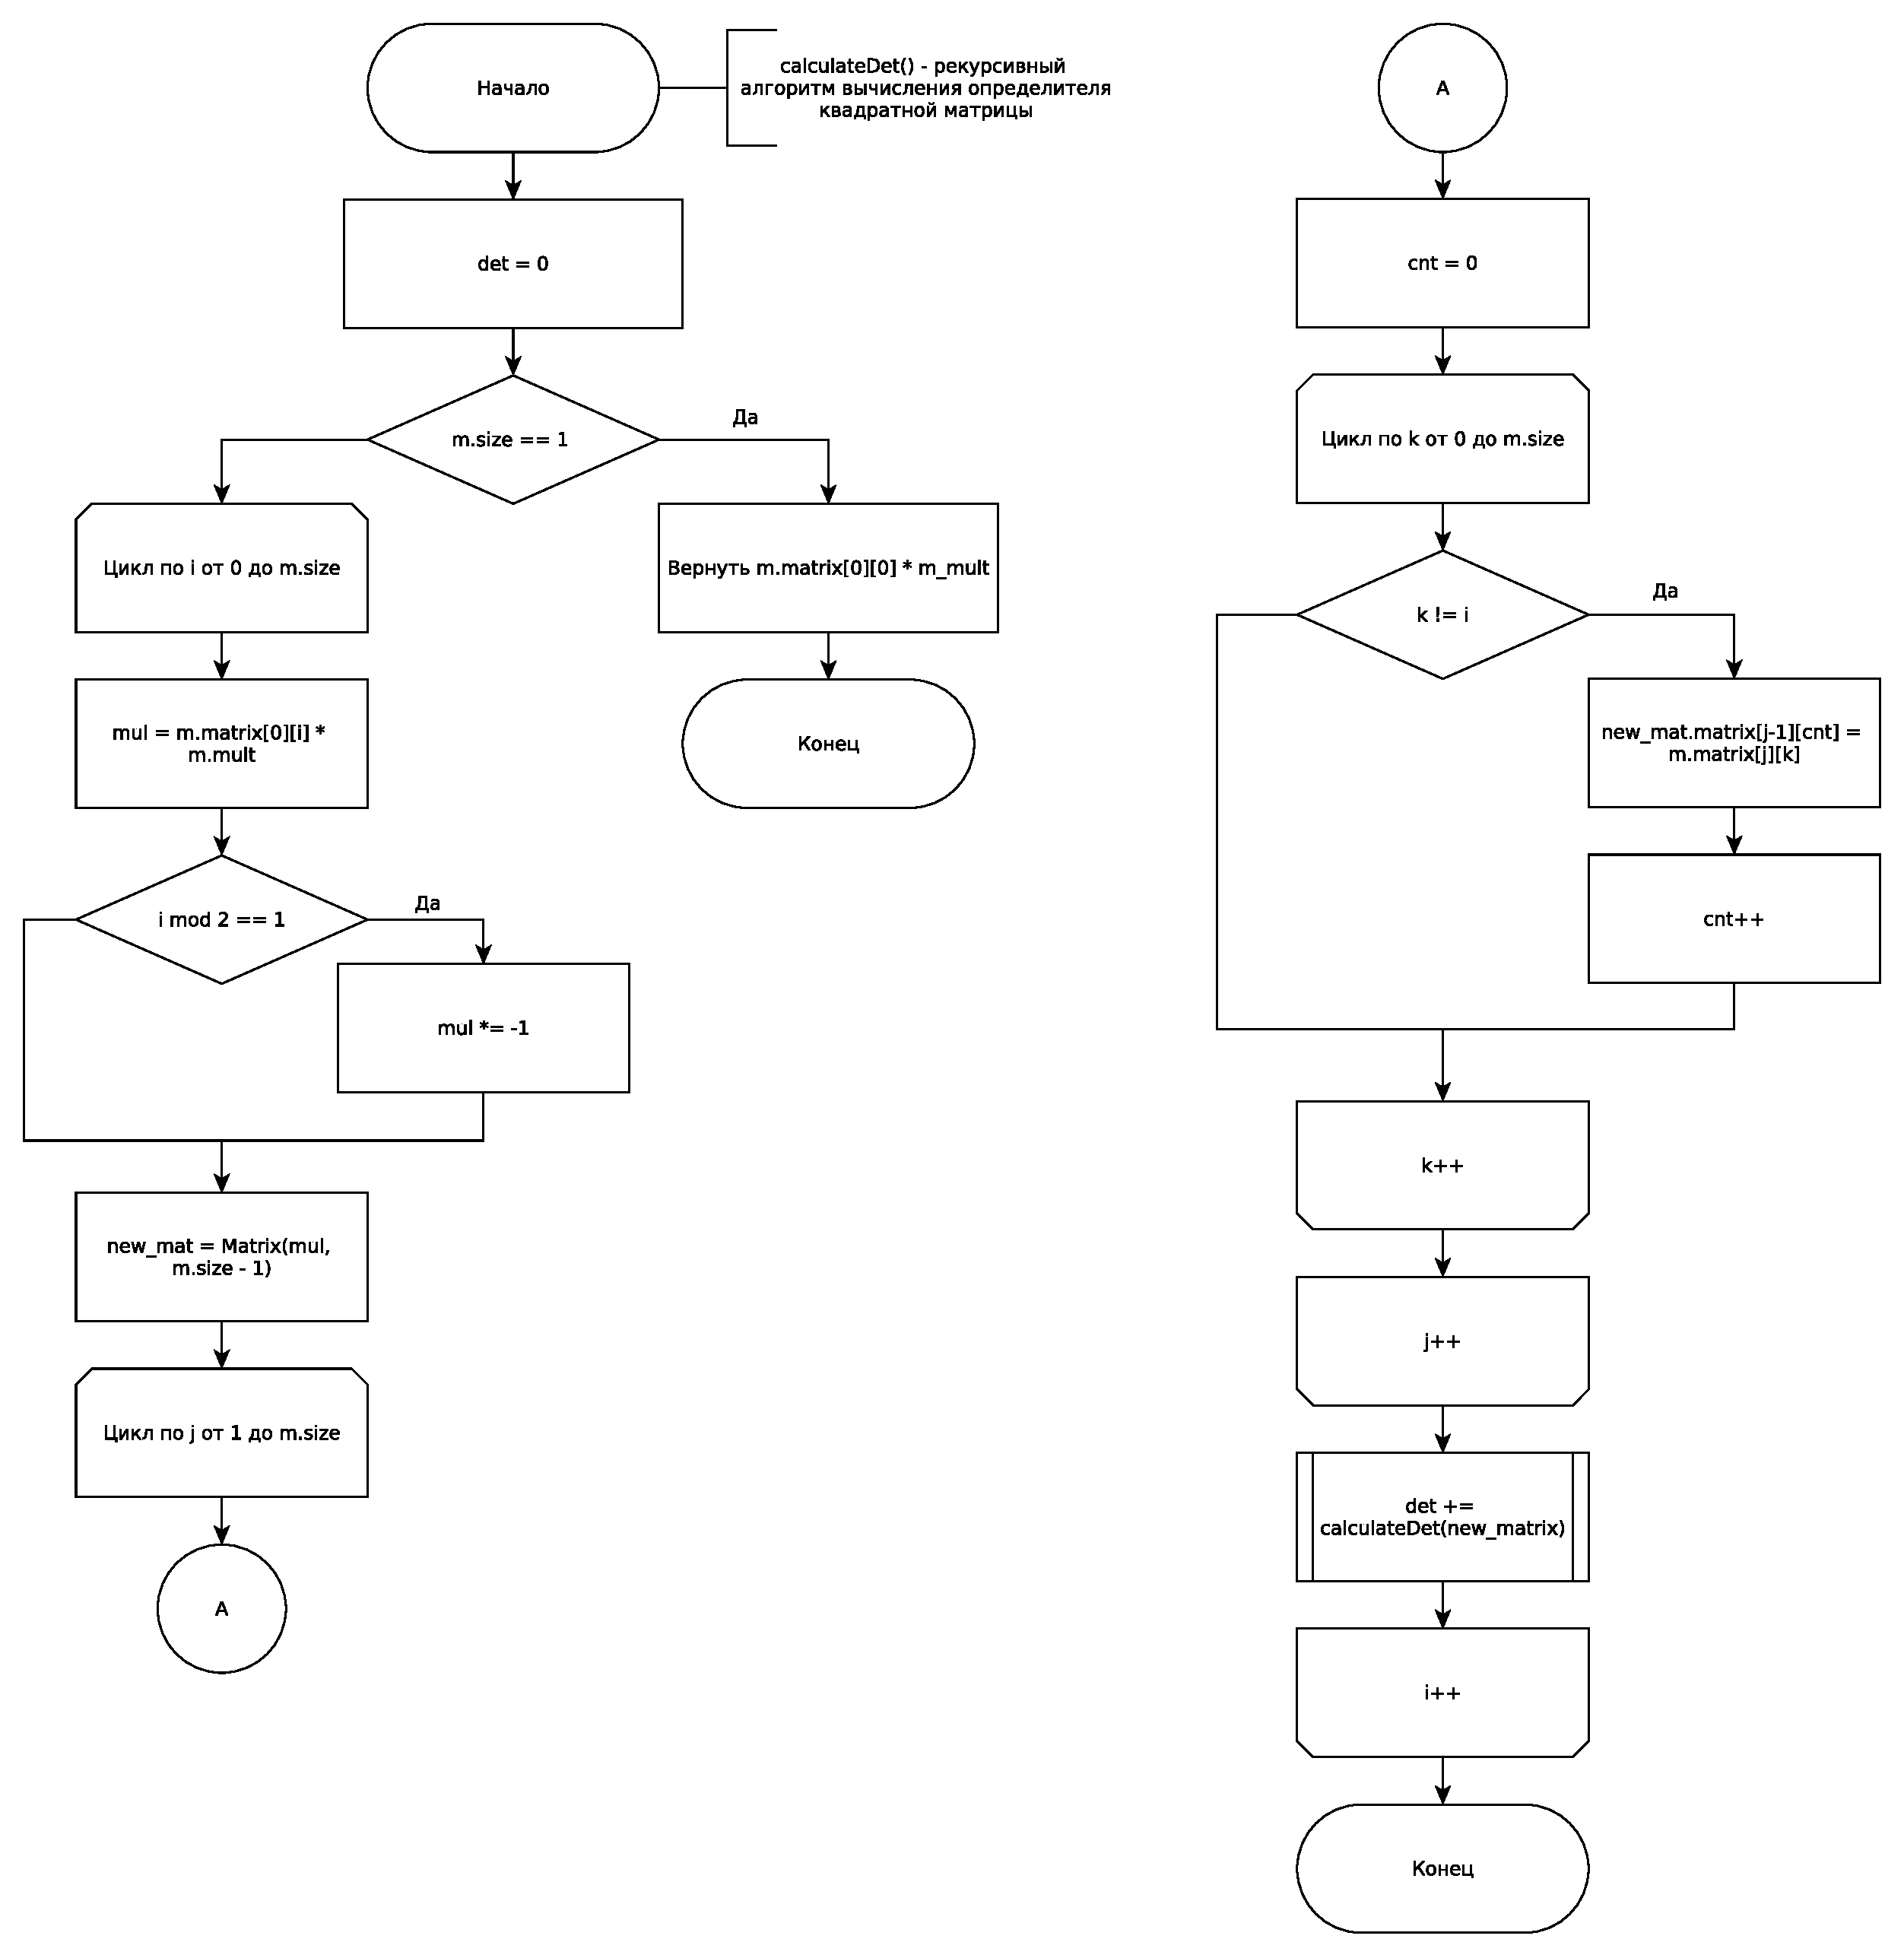
\includegraphics[width=1.00\linewidth]{img/count_det}
    	\caption{Схема организации конвейера с тремя лентами}
    	\label{img:count_det}
    \end{figure}
    
    На рисунке~\ref{img:thread_schema} представлена схема последовательного алгоритма шифрования и сохранения паролей.
    
    \begin{figure}[H]
    	\centering
    	\includegraphics[width=0.85\linewidth]{img/thread_schema}
    	\caption{Схема последовательного алгоритма}
    	\label{img:thread_schema}
    \end{figure}
    
    На рисунках~\ref{img:solver_1} -~\ref{img:solver_2} представлена схема реализация алгоритма шифрования на конвейере с тремя лентами.
    
    \begin{figure}[H]
    	\centering
    	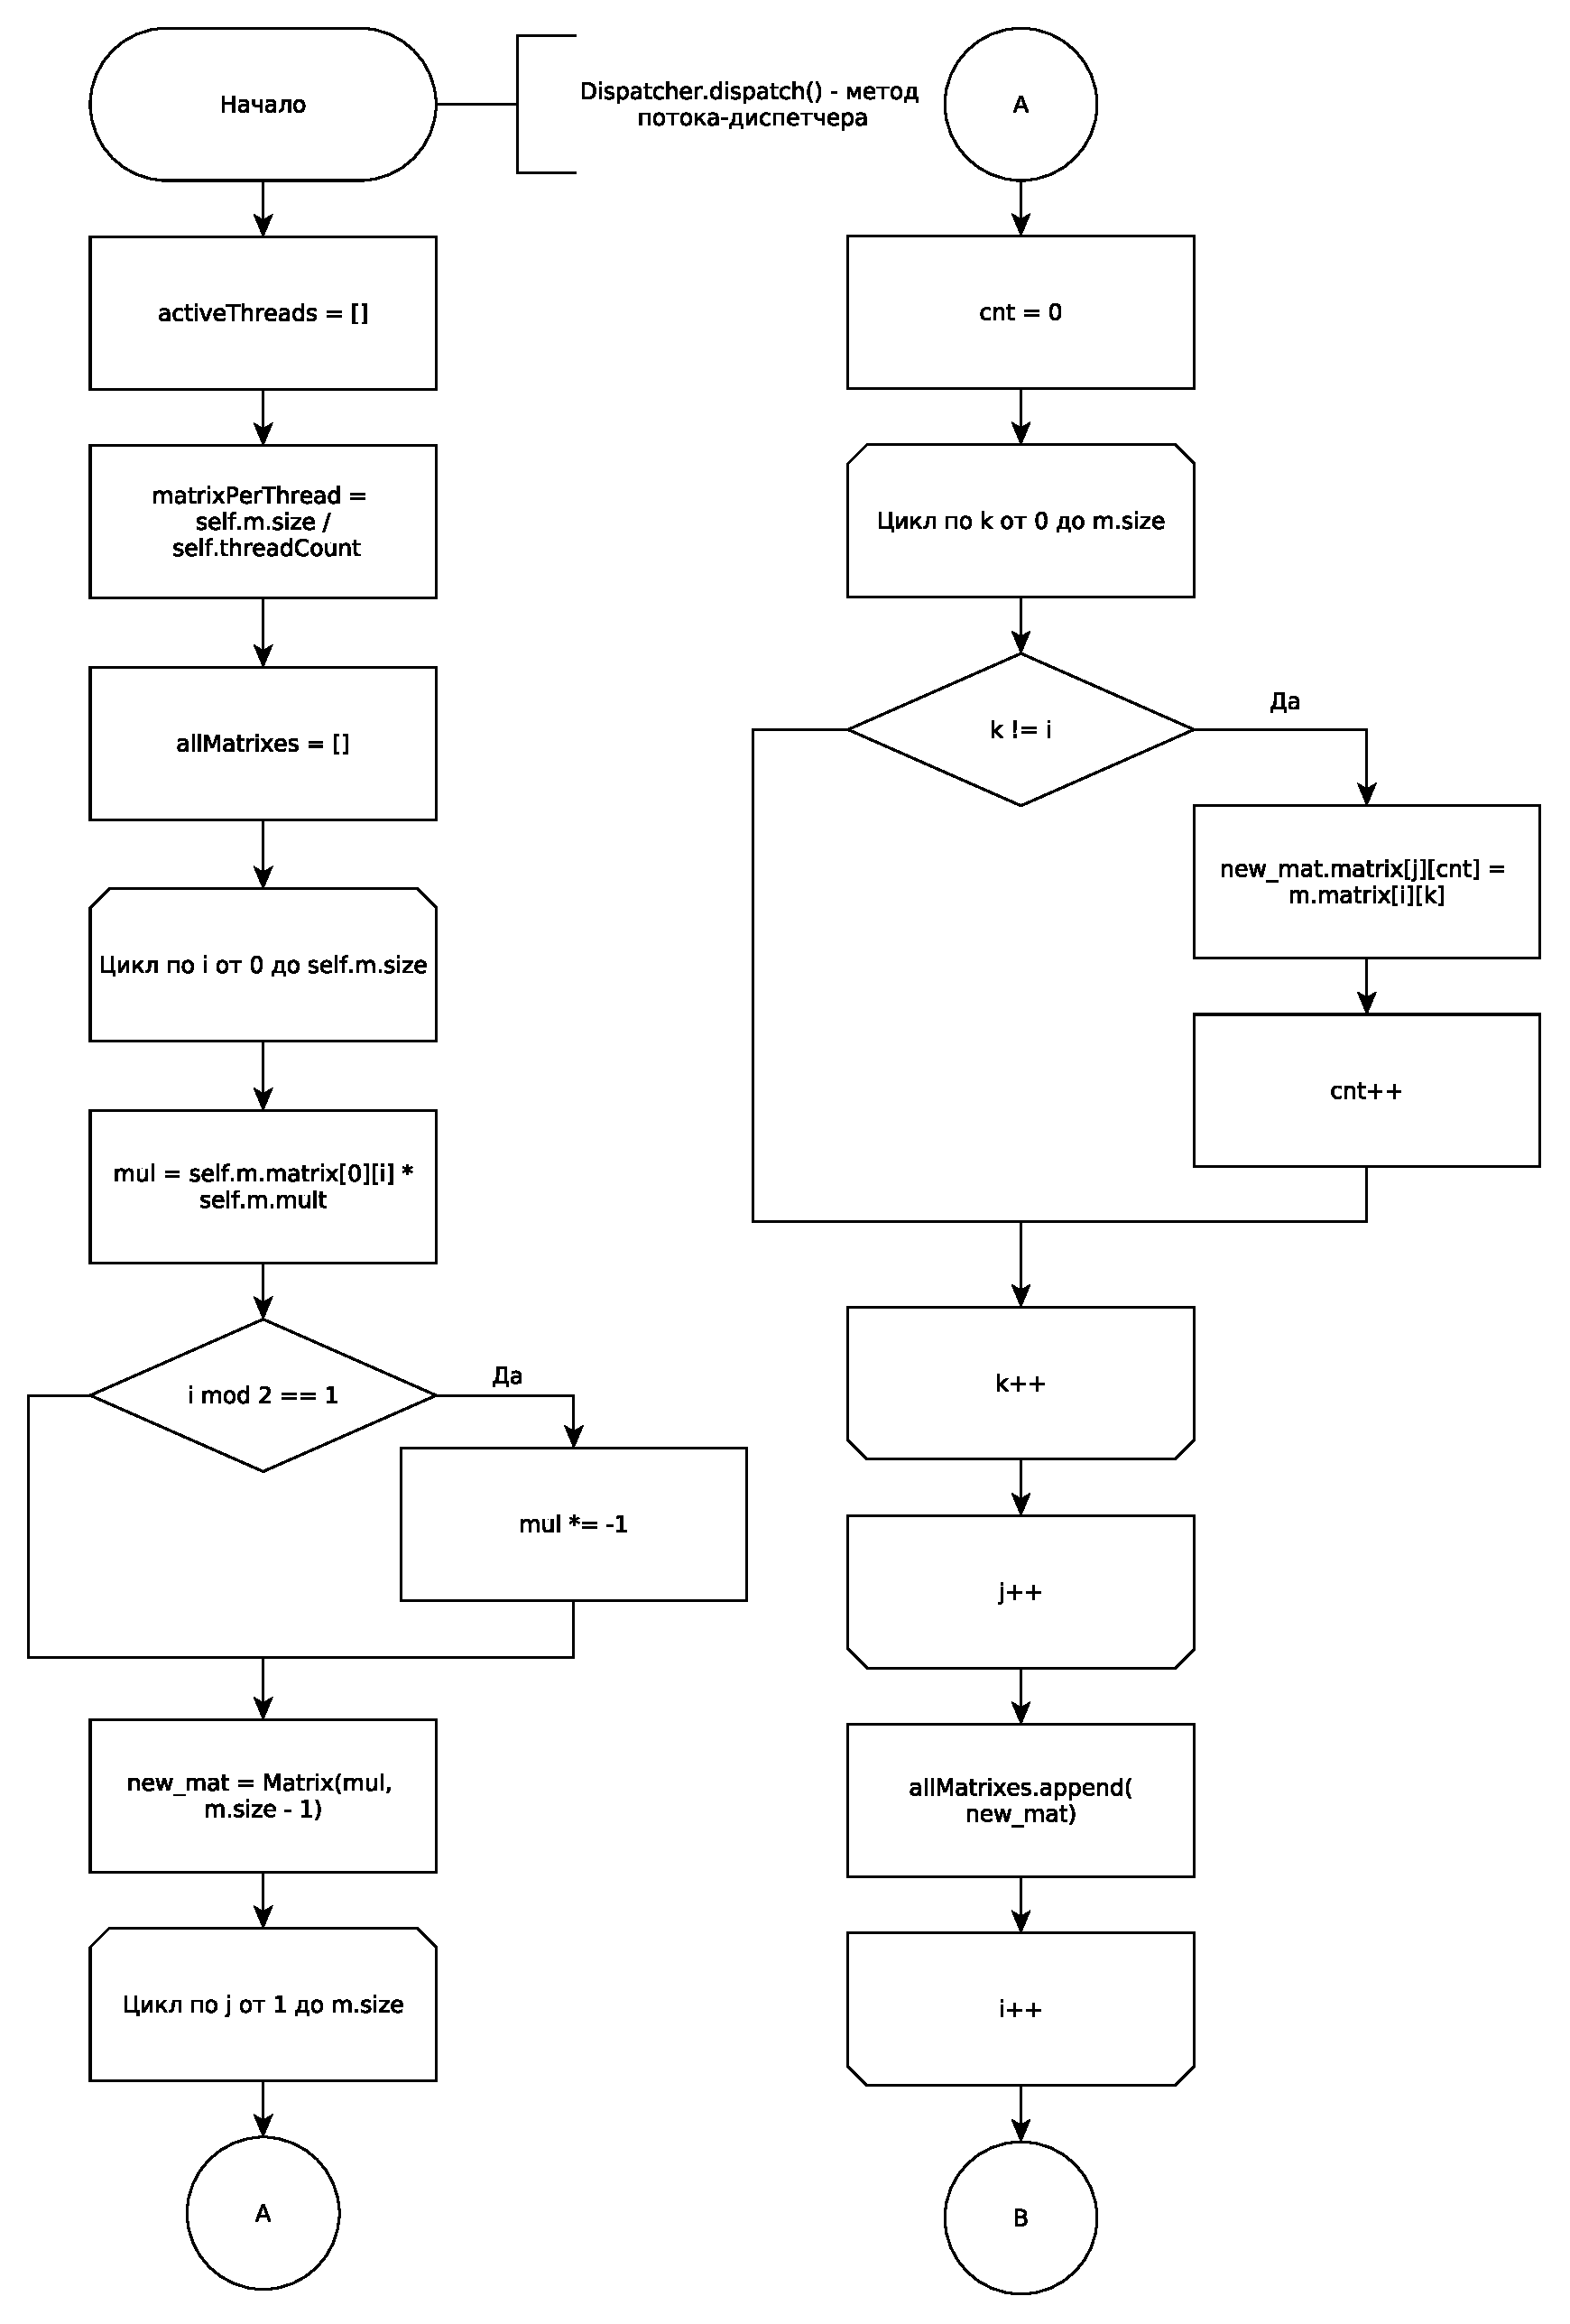
\includegraphics[width=0.85\linewidth]{img/solver_part_1}
    	\caption{Схема алгоритма работы конвейерной обработки}
    	\label{img:solver_1}
    \end{figure}
    
    \section{Структуры данных}
    Для удобства работы были выделены следующие классы:
    \begin{itemize}
    	\item UserStats со следующими полями:
    	\begin{itemize}
    		\item login - строка, логин пользователя
    	\end{itemize}
    	\item mul - множитель минора (целое число, 1 для четных столбцов, -1 для нечетных с учетом начала нумерации с нуля);
    	\item size - размер матрицы (целое число).
    \end{itemize}
    
    Для возможности генерации матриц, заполненных случайными элементами, класс Matrix содержит метод randomize.
    
    Для управления потоками выделен класс Dispatcher со следующими полями:
    \begin{itemize}
    	\item m - матрица вещественных чисел, определитель которой необходимо вычислить;
    	\item size - размер матрицы (целое число);
    	\item threadCount - количество создаваемых потоков;
    	\item returnList - список, разделяемый потоками, содержащий промежуточные вычисления определителей.
    \end{itemize}
    

    \subsection{Теоретический рассчет эффективности по времени}

    При параллельном выполнении алгоритма изначальная матрица размером $n \times n$ делится на $n$ матриц
    со значением $mult = (-1)^{j + 1} \cdot a_{1j}$,
    где $j$ - номер элемента в первом ряду, для которого находится значение минора.
    Далее "подматрицы" равномерно распределяются между потоками для вычисления значения миноров.
    По мере работы потоки записывают результат в общий массив, и после окончания работы всех потоков
    определитель исходной матрицы считается как сумма элементов в общем массиве.

    При таком методе распараллеливания алгоритма для матрицы размером $n \times n$ эффективность
    алгоритма по времени исполнения должна повышаться примерно в $k$ раз, где $k$ - количество потоков,
    при $1 < k \leq n / 2$ или $k = n$.
    Однако при $ n / 2 < k < n$, время исполнения алгоритма не увеличится более чем в $n / 2$ раза,
    так как часть потоков будут искать два слагаемых итогового определителя, а часть - одно,
    в таком случае произойдет простой второй части потоков.


    \section{Вывод}
    В данном разделе на основе приведенных в аналитическом разделе теоретических данных
    были составлены схемы алгоритмов для реализации в технологической части.
    Были составлены схемы разделения вычисления определителя на потоки.
    Проведены теоретические расчеты эффективности параллельного алгоритма нахождения определителя.
    \newpage


    \chapter{Технологическая часть}
    Данный раздел содержит обоснование выбора языка и среды разработки, реализацию алгоритмов.


    \section{Средства реализации}
    Для реализации программы был выбран язык программирования Python~\cite{Python}.
    Такой выбор обусловлен следующими причинами:
    \begin{itemize}
        \item удобные средства для работы с потоками;
        \item обладает информативной документацией.
    \end{itemize}


    \section{Реализация алгоритмов}
    В листингах~\ref{code:normal} -~\ref{code:parallel} представлены
    реализации рассматриваемых алгоритмов.

    \begin{lstlisting}[caption=Рекурсивный алгоритм, label={code:normal}]
        def calculateSum(m: Matrix):
    s = 0
    if m.size == 2:
        return (m.matrix[0][0] * m.matrix[1][1] - m.matrix[0][1] * m.matrix[1][0]) * m.mult

    for i in range(m.size):
        mul = m.matrix[0][i] * m.mult
        if i % 2 == 1:
            mul *= -1

        size = m.size - 1
        matrix = []

        for j in range(1, m.size):
            matrix.append([])
            for k in range(m.size):
                if k != i:
                    matrix[-1].append(m.matrix[j][k])

        s += calculateSum(Matrix(size, mul, matrix))
    return s
    \end{lstlisting}

    \begin{lstlisting}[caption=Параллельный алгоритм с делением на потоки\, класс Solver и функция calculateSumThreading,
        label={code:parallel}]
        def calculateSumThreading(matrixes, returnList: list):
    t = time.time()
    s = 0

    for m in matrixes:
        if m.size == 2:
            returnList.append((m.matrix[0][0] * m.matrix[1][1] - m.matrix[0][1] * m.matrix[1][0]) * m.mult)
            continue

        for i in range(m.size):
            mul = m.matrix[0][i] * m.mult
            if i % 2 == 1:
                mul *= -1

            size = m.size - 1
            matrix = []

            for j in range(1, m.size):
                matrix.append([])
                for k in range(m.size):
                    if k != i:
                        matrix[-1].append(m.matrix[j][k])

            s += calculateSum(Matrix(size, mul, matrix))
            # allMatrixes.append(Matrix(size, mul, matrix))

    returnList.append(s)
    # print(f'process {getpid()}, time {time.time() - t}')

class Solver:
    def __init__(self, matrix: Matrix = None):
        self.m = matrix
        if self.m is None:
            self.m = Matrix(10).randomize()

        self.threadCount = 1
        self.threadManager = Manager()
        self.returnList = self.threadManager.list()


    def solve(self):
        activeThreads = []
        matrixPerThread = self.m.size / self.threadCount
        allMatrixes = []

        for i in range(self.m.size):
            mul = self.m.matrix[0][i] * self.m.mult
            if i % 2 == 1:
                mul *= -1

            size = self.m.size - 1
            matrix = []

            for j in range(1, self.m.size):
                matrix.append([])
                for k in range(self.m.size):
                    if k != i:
                        matrix[-1].append(self.m.matrix[j][k])

            allMatrixes.append(Matrix(size, mul, matrix))

        startMatrix = 0
        threadTasksCount = []

        for i in range(self.threadCount):
            endMatrix = round(matrixPerThread * (i+1))
            # if endMatrix == startMatrix: break
            if i == self.threadCount - 1:
                threadMatrixes = allMatrixes[startMatrix:]
            else:
                threadMatrixes = allMatrixes[startMatrix:endMatrix]
            startMatrix = endMatrix
            activeThreads.append(
                Process(target=calculateSumThreading, args=(threadMatrixes, self.returnList,)))
            threadTasksCount.append(len(threadMatrixes))

        for thread in activeThreads:
            thread.start()
        for thread in activeThreads:
            thread.join()
        self.returnList = self.threadManager.list()

        return sum(self.returnList)
    \end{lstlisting}


    \section{Тестирование}
    В таблице~\ref{tab:tests} представлены использованные для тестирования методом "черного ящика" данные,
    были рассмотрены все возможные тестовые случаи.
    Все тесты пройдены успешно.

    \begin{table}[H]
        \begin{center}
            \captionsetup{justification=raggedright, singlelinecheck=false}
            \caption[]{\label{tab:tests} Проведенные тесты}

            \begin{tabular}{|c|c|}
                \hline
                \rule[-1ex]{0pt}{2.5ex} Матрица & Определитель \\
                \hline
                \rule[-1ex]{0pt}{2.5ex} $\begin{pmatrix}
                                             0 & 0 \\
                                             0 & 0
                \end{pmatrix}$ & 0
                \\
                \hline
                \rule[-1ex]{0pt}{2.5ex} $\begin{pmatrix}
                                             1 & 0 & 0 \\
                                             0 & 1 & 0 \\
                                             0 & 0 & 1
                \end{pmatrix}$ & 1
                \\
                \hline
                \rule[-1ex]{0pt}{2.5ex}    $\begin{pmatrix}
                                                1 & 2 & 3  \\
                                                4 & 5 & 6  \\
                                                7 & 8 & 12
                \end{pmatrix}$ & -9
                \\
                \hline
                \rule[-1ex]{0pt}{2.5ex} $\begin{pmatrix}
                                             1  & 2  & 3  & 4  \\
                                             5  & 6  & 7  & 8  \\
                                             9  & 10 & 11 & 12 \\
                                             13 & 14 & 15 & 16
                \end{pmatrix}$ & 0
                \\
                \hline
            \end{tabular}
        \end{center}
    \end{table}


    \section{Вывод}
    В данном разделе были реализованы и протестированы алгоритмы нахождения определителя матрицы:
    обычный и параллельный.
    \newpage


    \chapter{Экспериментальная часть}
    В данном разделе сравниваются реализованные алгоритмы, дается сравнительная оценка затрат по времени.


    \section{Пример работы программы}
    Пример работы программы представлен на рисунках.
    


    \section{Технические характеристики}
    Технические характеристики устройства, на котором выполнялось тестирование:
    \begin{itemize}
        \item операционная система --- Windows~\cite{windows} 10 64-bit;
        \item оперативная память --- 16 Гб;
        \item процессор --- Intel(R) Core(TM) i5-7600 CPU @ 3.50GHz~\cite{i5}.
    \end{itemize}


    \section{Время выполнения алгоритмов}

    Время выполнения алгоритмов замерялось на автоматически генерируемых
    квадратных матрицах необходимого размера с использованием функции getrusage библиотеки resources.

    \begin{table}[h]
        \begin{center}
            \captionsetup{justification=raggedright, singlelinecheck=false}
            \caption{\label{time} Время нахождения определителя матрицы при
            использовании разного количества потоков в микросекундах}
            \begin{tabular}{|c c c c c c c|}
                \hline
                Размерность & 1 п. & 2 п. & 4 п. & 8 п. & 16 п. & 32 п.
                \\
                \hline
                4 & 10  & 14  & 17  & 23  & 38  & 67  \\
                \hline
                5 & 10  & 14  & 17  & 23  & 38  & 68  \\
                \hline
                6 & 12  & 15  & 17  & 24  & 39  & 68  \\
                \hline
                7 & 22  & 19  & 21  & 25  & 40  & 72  \\
                \hline
                8 & 75  & 47  & 37  & 42  & 57  & 82  \\
                \hline
                9 & 529 & 306 & 304 & 164 & 155 & 182 \\
                \hline
            \end{tabular}
        \end{center}
    \end{table}

    На рисунке~\ref{img:graph} графически изображена зависимость
    времени работы алгоритма от размерности матрицы и количества потоков.

    \begin{figure}[H]
        \centering
        \includegraphics[width=0.8\linewidth]{img/graph}
        \caption{
            Зависимость времени работы алгоритма от размерности матрицы и количества потоков
        }
        \label{img:graph}
    \end{figure}

    Поскольку процессор на устройстве содержит 4 физических и логических ядра,
    эффективность алгоритма улучшается только при создании 4 и менее потоков.
    Как видно по графику~\ref{img:graph}, с 2 потоками алгоритм выполнялся практически
    в 2 раза быстрее, чем с 1 потоком.
    Аналогичная ситуация наблюдается при сравнении 4 и 2 потоков.


    \section{Вывод}
    В данном разделе были проведены измерения времени, требуемого на исполнение алгоритма.
    По результатам измерений видно, что с увеличением количества потоков скорость выполнения
    алгоритма увеличивается.
    Однако как только количество потоков становится равно количеству логических ядер процессора,
    временные затраты на выполнение алгоритма увеличиваются из-за времени, затрачиваемого на
    создание новых потоков.


    \newpage

    \addcontentsline{toc}{chapter}{Заключение}
    \chapter*{Заключение}
    В процессе выполнения лабораторной работы были изучены и реализованы последовательный и
    параллельный рекурсивные алгоритмы нахождения определителя матрицы.

    Было экспериментально вычислено реальное время выполнения выше обозначенных алгоритмов.
    В результате было выявлено, что распараллеливание алгоритма нахождения определителя
    матрицы позволяет увеличить скорость его выполнения при использовании количества потоков
    меньшего или равного количеству логических ядер процессора.


    \newpage
    \addcontentsline{toc}{chapter}{Литература}

    \bibliographystyle{utf8gost705u}  % стилевой файл для оформления по ГОСТу
    \bibliography{report_4}          % имя библиографической базы (bib-файла)

\end{document}